\chapter{イントロダクション}
\label{chap1}

\section{システムのディペンダビリティ:基礎概念と現代的課題}

\subsection{システムとは何か}

私たちの日常生活において、「システム」という言葉をよく耳にします。しかし、この概念を正確に定義するのは簡単ではありません。ここでは、参考文献[x]の定義を示します。

システム: 他のシステムと相互作用するもの。ここでいうシステムは、与えられた環境であり、ハードウェア、ソフトウェア、人間、および自然現象を伴う物質的世界などである。システム境界はシステムとその環境が接する境目である。

システムは互いにサービスを介して相互作用を行います。参考文献[x]のサービスの定義を示します。

サービス:システムが(提供者の役割によって)提供するサービスとは、その利用者から見える振る舞いです。ここで利用者とは、提供者からサービスを受ける別のシステムです。提供者のシステム境界のうちサービス提供がなされる部分を提供者のサービスインタフェースといいます。

システムは常に特定の環境に置かれており、その環境との相互作用を通じて機能します。例えば、自動車というシステムは道路という環境の中で機能し、気象条件や交通状況などの環境要因の影響を受けます。

システムとサービス、および環境の関係を図\ref{fig:system1}に示します。
\begin{figure}[htbp]
\centering
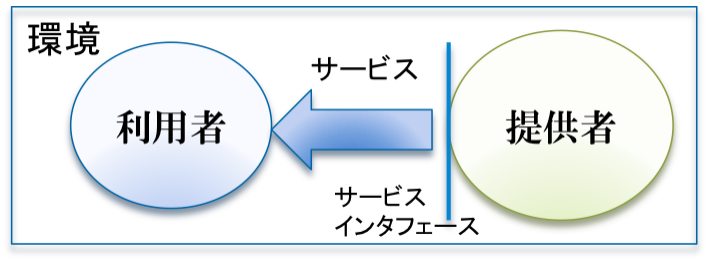
\includegraphics[width=\textwidth]{safety_assurance_contents/ch1images/system_environment.pdf}
\caption{環境におけるシステムとサービス}
\label{fig:system1}
\end{figure}

上記の定義は抽象的ですが、サービスは、システムによって私たちに提供される機能や便益です。私たちユーザーは、このサービスを通じてシステムと関係を持ちます。例えば、スマートフォンというシステムは、通話、メッセージング、インターネット閲覧などのサービスを提供し、私たちはこれらのサービスを通じてスマートフォンと関わっています。

\subsection{ディペンダビリティの概念}
`ディペンダビリティ(Dependability)は、直訳すると「依存可能性」となりますが、システム工学では「総合信頼性」と訳されることが多い重要な概念です。この概念の起源は、あるシステムが別のシステムに依存(Depend)することができる、そのシステムの性質を表すことにあります。

例えば、運転手(システムA)が自動車(システムB)に依存する場合を考えてみましょう。自動車がディペンダブル(依存可能)であるためには、どのような性質を持つべきでしょうか?安全であること、運転しやすいこと、目的地まで確実に到達できることなどが挙げられるでしょう。このように、ディペンダビリティは利用者や環境によって求められる性質が異なる、相対的な概念です。

ディペンダビリティは、日本語では現在「総合信頼性」と呼ばれています。以下にいくつかの定義を示します。

\begin{itemize}
\item 容認できる以上の頻度と深刻さのサービス障害を防ぐシステムの能力
\item 可用性性能及びこれに影響を与える要因、すなわち信頼性性能、保全性性能及び保全支援能力を記述するために用いられる包括的な用語(JIS Z 8115)
\end{itemize}

ディペンダビリティはJIS Z 8115などにおけるように、可用性や信頼性など、従来のシステムの非機能要求を総合したものとして考えられてきました。しかし、もともとはシステム間の依存関係に由来し、サービス障害などに関連する概念です。可用性や信頼性は、システムがディペンダブルであるためには必要な非機能要求であると考えられますが、システムは環境に置かれ、また利用者によってサービスは使用されるため、必要となる機能、非機能などは環境や利用者によって異なります。またディペンダブルであるために必要となる機能や非機能が提供されなくなった場合、つまりシステムに障害が発生した場合、システムは復旧を行い、サービスを継続し無くてはなりません。

以上をまとめるとシステムがディペンダブルであるためには、以下の条件を満たす必要があります:

\begin{itemize}
\item 利用者や環境において望まれる性質を持ち続けること
\item サービスを継続的に提供すること
\end{itemize}

これらを満たすためには、システムがその性質を失った場合(つまり、ディペンダブルでなくなった場合)には、速やかに復旧を行い、サービスを継続する能力も求められます。

\section{ディペンダビリティの体系と用語}

ディペンダビリティの概念は、1980年代から国際的な研究グループ(IFIP WG 10.4 ``Dependable Computing and Fault Tolerance"など)によって体系化され、用語の整理が行われてきました。当初は「耐故障性(Fault Tolerance)」研究から発展し、近年ではセキュリティの概念も含めて議論されています。

ここでは、Avizienis et al. (2004)による体系に基づいて、ディペンダビリティの主要な概念を紹介します。

\subsection{ディペンダビリティ属性}

ディペンダビリティ属性は、システムがディペンダブルであるために持つべき特性を表します。主な属性には以下のものがあります:

\begin{itemize}
\item 可用性(Availability):正しいサービスの即応性
\item 信頼性(Reliability):正しいサービスの継続性
\item 安全性(Safety):利用者と環境へ破壊的影響をもたらさないこと
\item 一貫性(Integrity):不適切なシステム変更がないこと
\item 保守性(Maintainability):変更と修理を受け入れられること
\end{itemize}

これらの属性は相互に関連しており、時には相反する関係にあることもあります。システム設計者は、対象システムの要求に応じてこれらの属性のバランスを取る必要があります。

\subsection{ディペンダビリティへの脅威}

システムのディペンダビリティを脅かす要因は、以下の3つの概念で整理されています:

\begin{itemize}
\item 欠陥(Fault):エラーの原因となるとみなされる、あるいは推定されるもの、こと
\item 誤り(Error):障害が起こりうるシステムの状態(ただし、エラー状態になったからといって、必ずしも障害が起こるとは限らない)
\item 障害(Failure):サービスが正しいサービスから逸脱する出来事
\end{itemize}

これらの概念は因果関係にあり、欠陥がエラーを引き起こし、エラーが障害につながる可能性があります。

\subsection{ディペンダビリティへの脅威に対処する手段}

ディペンダビリティへの脅威に対処するため、以下の4つの手段が提案されています:
\begin{itemize}
\item 欠陥防止(Fault Prevention):欠陥の導入や発生を防ぐ
\item 耐故障性(Fault Tolerance):欠陥がある中で障害を防ぐ
\item 欠陥除去(Fault Removal):欠陥の数や深刻度を減らす
\item 欠陥予測(Fault Forecasting):欠陥の現在の数、今後の障害、影響などを予測する
\end{itemize}

ディペンダビリティの属性、脅威、対処手段をまとめると図Xのディペンダビリティとセキュリティの木になります。ディペンダビリティとセキュリティは、システムのあるべき姿に関する概念であり、図Xはシステムのあるべき姿に関する研究成果の一つと言えます。

% 図 ディペンダビリティとセキュリティの木

%これらの手段を適切に組み合わせることで、システムのディペンダビリティを向上させることができます。

\section{現代のシステムとディペンダビリティの課題}

IT・組込みシステムの重要性が増すにつれ、ITシステムは私たちの生活および社会において欠かせないインフラとなり、さらにポータル化してきました。私たちの生活、そして社会は便利になりましたが、同時に従来のディペンダビリティや耐故障性の考え方だけでは対処できない問題が増えてきました。これらの問題は以下のようにまとめられます(参考文献[2])。
\begin{itemize}
\item システムの大規模化による問題
\item プログラムサイズの巨大化
\item 多機能化
\item ブラックボックス化したコンポーネント
\item 複雑化
\item 環境の変化による問題
\item 技術の急速な進化へのキャッチアップの困難さ
\item 接続システムの多様化
\item 利害関係者(Stakeholder)の変化による問題
\item 要求の頻繁な変更
\item 要求や合意に対する考え方の違い
\end{itemize}

これらは従来から問題とされてきたものですが、情報システムの規模が著しく拡大したことで、私たちはこれらの問題に対応できなくなりつつあるかもしれません。近年、深刻な情報システムの障害が報告されています。例えば、2012年6月に発生したレンタルサーバでの5000を超える企業データ消失問題では、復旧作業中に顧客データが他の顧客に流出するなど、さまざまな混乱が生じました(朝日新聞2012年7月7日)。

情報システムの規模が拡大する中で、私たちはシステムのディペンダビリティを従来通りにコントロールすることが難しい状況に直面しているかもしれません。では、どうすればよいのでしょうか。従来の耐故障技術、テスト、より精密な形式手法などは、これからますます重要になると考えられます。しかし、情報システムの規模が拡大し続ける中では、このアプローチだけでは限界があると考えます。つまり、障害を完全に回避することは難しいのです。私たちは、障害は完全には防げないという前提に立って、今後のディペンダビリティを考察しました(参考文献[3][4])。

ディペンダビリティは、可用性や信頼性とは異なり、利用者を中心とした概念といえます。利用者や利害関係者に、障害が完全に防げなくてもディペンダブルであると感じてもらうにはどうすればよいでしょうか。私たちは以下の点が重要であると考えます。

\begin{itemize}
\item システム保証(System Assurance):システムの安全性やディペンダビリティを利用者などの利害関係者に説明し、納得してもらうこと。
\item 説明責任達成(Accountability Achievement):システム開発や運用に際して、利用者などの利害関係者に必要な説明を正しく行うこと。特に障害が発生した場合には、その原因や事後対策、利用者への影響などを説明すること。
\end{itemize}

従来のディペンダビリティは、耐故障性など、主に工学的・技術的側面で研究されてきました。しかし、工学的・技術的なアプローチだけでは、今後のシステムのディペンダビリティを保つのは難しいかもしれません。そのため、他の手法も組み合わせる必要があります。私たちは、ディペンダビリティが利用者を重視した概念であることから、利用者や利害関係者に対するシステム保証と説明責任達成が重要であると考えました。

社会的にも、システム保証と説明責任の重要性は高まっています。例えば、2009年から2010年に問題となったアメリカでのトヨタ車リコール問題では、最終的にトヨタ車に欠陥がなかったと報告されたにもかかわらず、トヨタは大きな批判を浴びました。この問題は政治的な背景が強かったといわれていますが[1]、参考文献[5]は、トヨタに適切な説明体制が整っていなかったために問題が大きくなったと分析しています。また、2011年に発行された自動車の機能安全規格ISO26262について、参考文献[6]では「最大のインパクトは、安全性の根拠をより説明しやすくするよう自動車メーカーに求める点である」と指摘されています。ちなみに、ISO26262では、D-Caseのもとになったセーフティケースの提出が要求されています。

ディペンダビリティは、耐故障性の研究から始まり、安全性や信頼性を統合した概念として議論されてきました。しかし、近年のITシステムはあらゆる面で規模が拡大し続けており、そのディペンダビリティを達成するためには、従来の工学的アプローチだけでなく、システム保証や説明責任達成が重要であると考えています。本書で紹介するD-Caseは、その観点から出発したものです。


最近では、AI(人工知能)技術を用いたシステム、特に自動運転システムなどのディペンダビリティが重要な課題となっています。AI技術の不確実性や説明可能性の問題は、従来のシステムとは異なる新たなディペンダビリティの課題を提起しています。


システムのディペンダビリティは、もはや単なる技術的な問題ではなく、社会的、倫理的な問題としても捉えられるようになっています。システムの複雑化、不確実性の増大、そしてAI技術の台頭により、従来のディペンダビリティの概念や手法だけでは不十分になってきています。

これからのディペンダビリティ確保には、技術的な対策に加えて、システム保証と説明責任の遂行が不可欠です。また、不完全性や不確実性を前提としたシステム設計と運用の考え方を確立していく必要があります。

システム開発者、運用者、そして利用者を含むすべてのステークホルダーが、これらの課題を理解し、協力してディペンダブルなシステムの実現に取り組むことが求められています。

\section*{参考文献}
\begin{enumerate}
\item 
\end{enumerate}

